\documentclass{article}
\usepackage{amsmath}
\usepackage{amssymb}
\usepackage{graphicx}
\usepackage[margin=1in]{geometry}
\usepackage{hyperref}
\usepackage{caption}
\usepackage{float}
\graphicspath{{images/}}
\hypersetup{
  colorlinks=true,
  urlcolor=blue,
}
\begin{document}

\title{Game Notes}
\author{Aresh Pourkavoos}
\maketitle

Position within square stored as an odd signed integer in half-pixels,
e.g.
\begin{center}
  \begin{tabular}{|c|c|c|c|}
    \hline
    101 & 011 & 001 & 011 \\ \hline
    -3 & -1 & 1 & 3 \\ \hline
  \end{tabular}
\end{center}
Requires entities to have odd pixel dims to be centered \\
Edge/vertex states are not possible \\
Updating position requires doubling velocity first \\
Store position as $x$ and $y$ seen on screen
or relative to a square's axes? \\
Screen position: 
\begin{itemize}
\item
  Graphics and movement are easier
\item
  Collision would be most convenient by loading the current square rotated
\end{itemize}
Relative position:
\begin{itemize}
\item
  Collision is easier, just check against stored square
\item
  Need to ensure that rendering is done correctly
\end{itemize}
View splitting is decided by determinant sign:
will always give edge to cell further (counter?)clockwise \\
Vertices/edges are on the border between pixels (even position):
do not require a special case
\begin{center}
  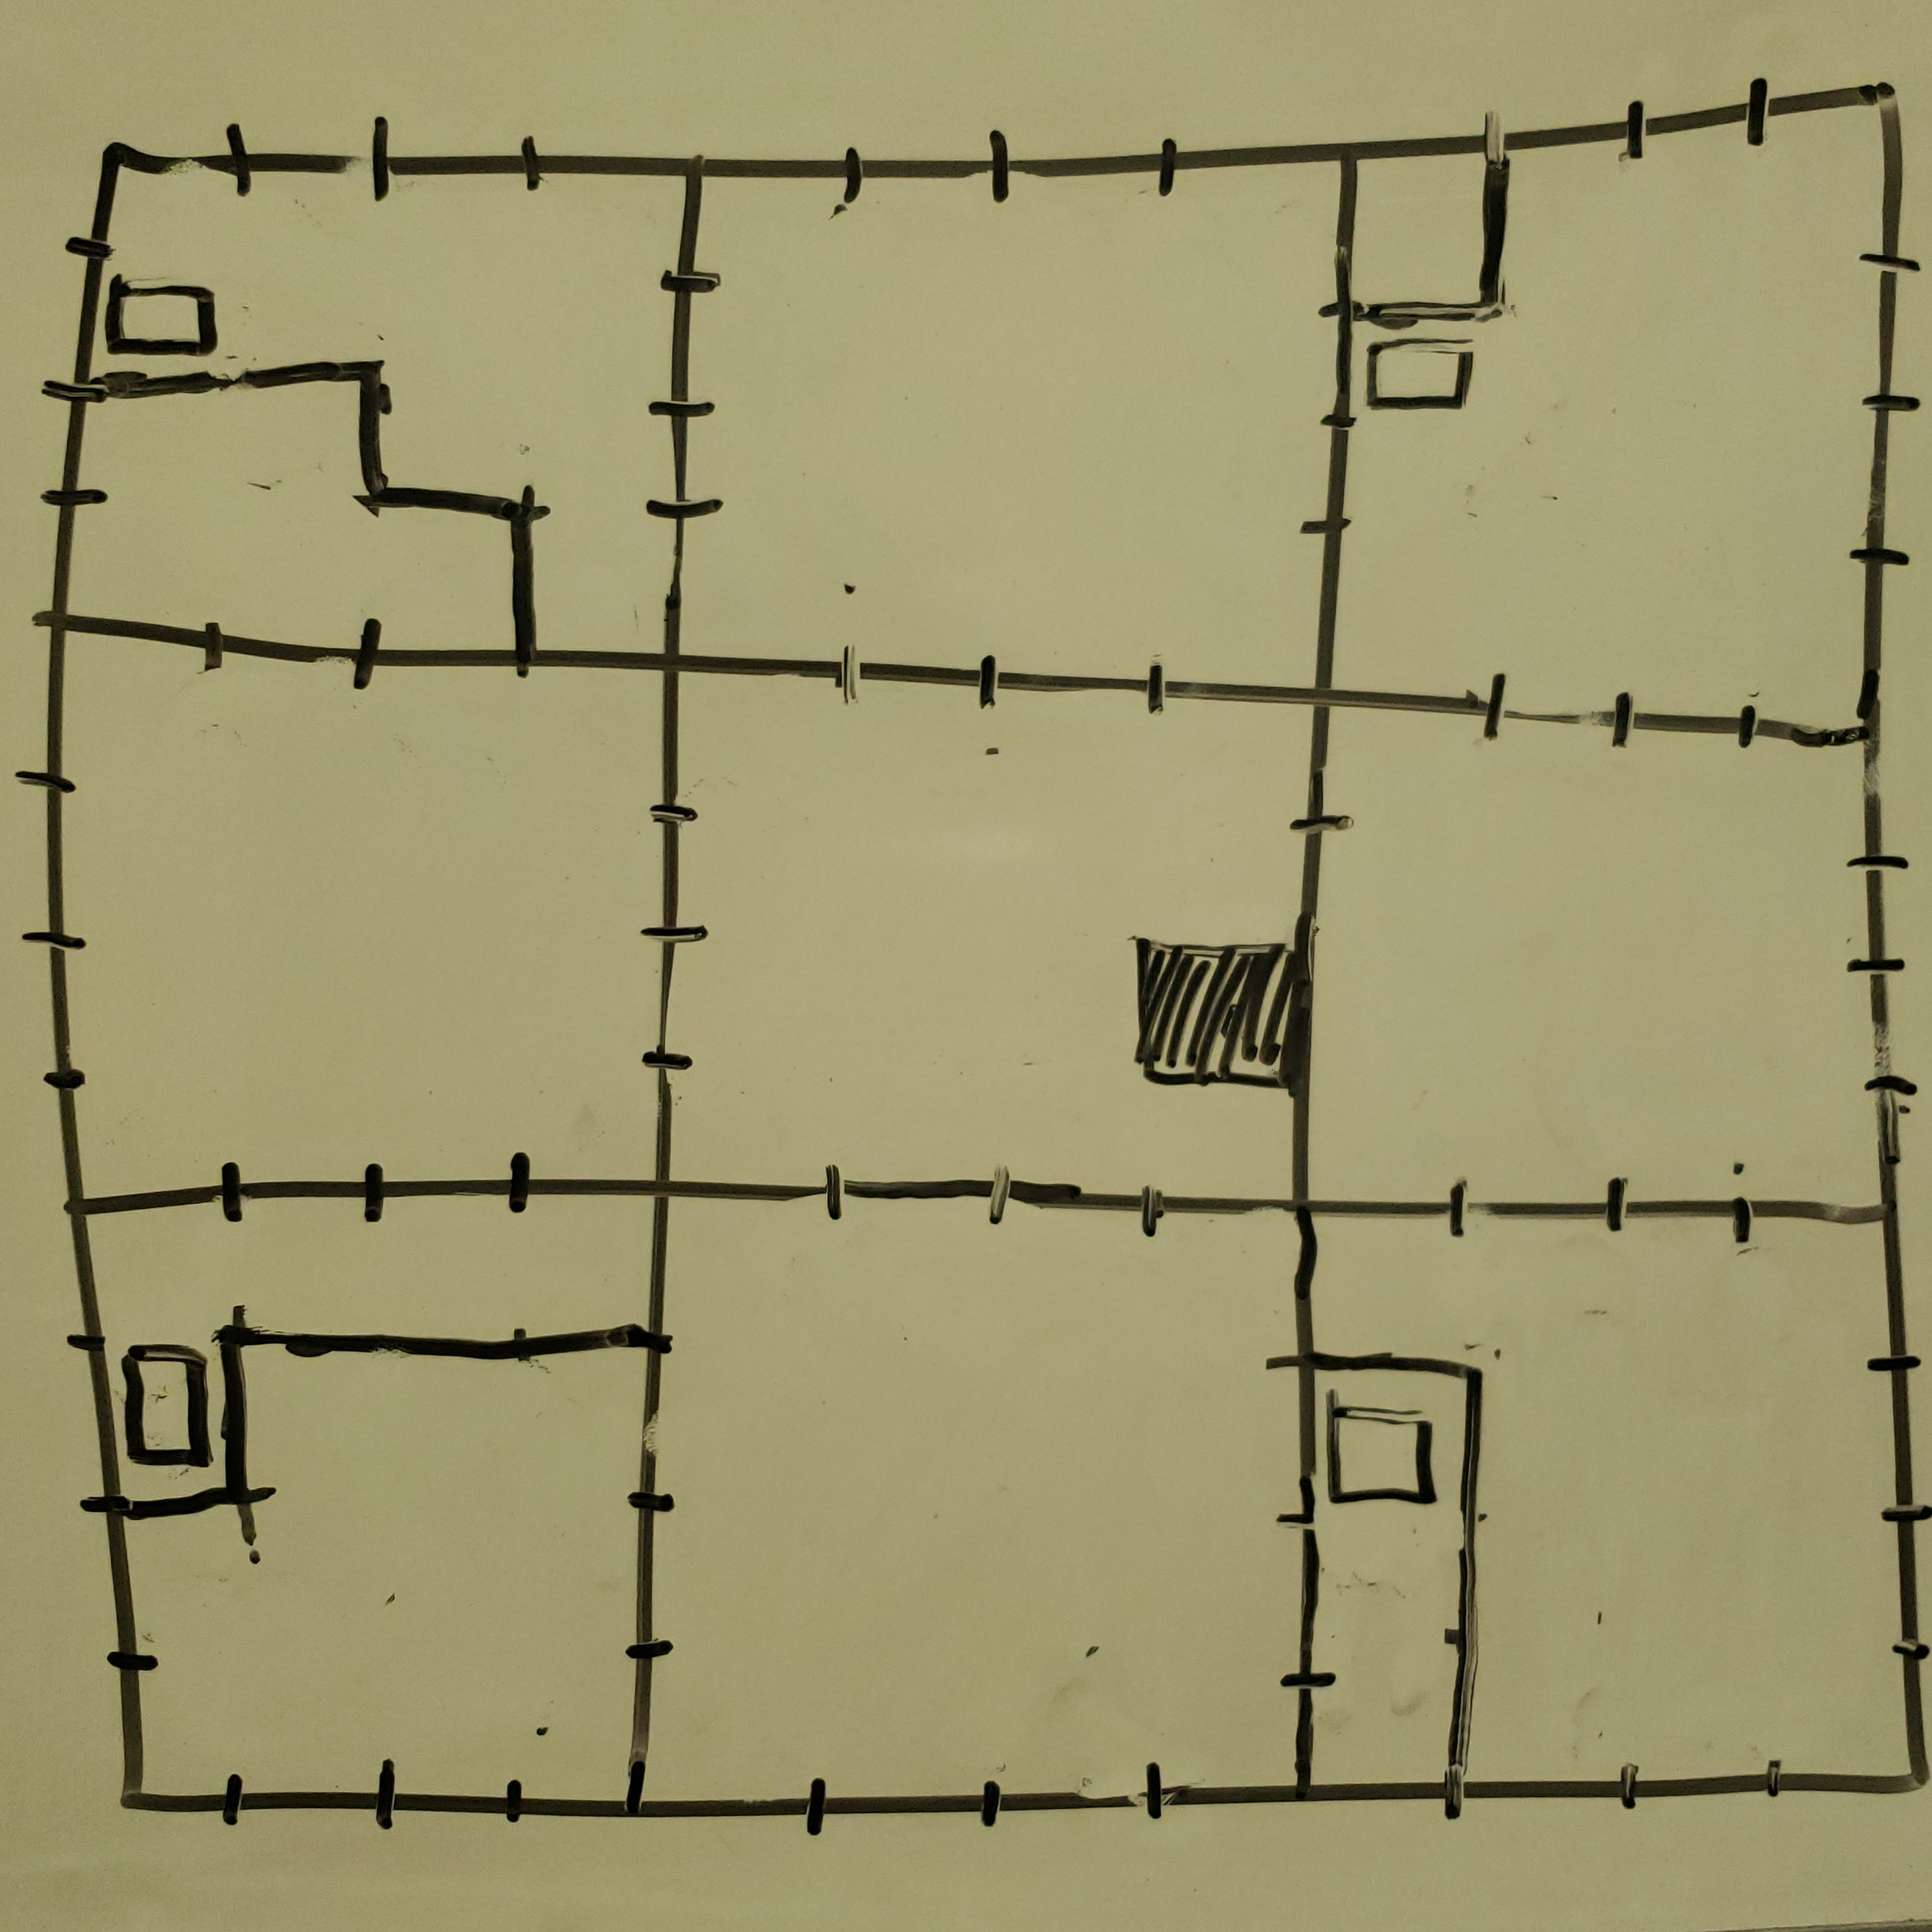
\includegraphics[width=0.5\linewidth]{grid.jpg}
\end{center}
Shaded pixel: camera \\
Lines: region boundaries \\
Inlined pixels: edge cases (given to clockwise region in this case) \\
Going through a singularity and back is a holonomy loop \\
Entity gravity is ambiguous when not in the same square as the player:
\begin{itemize}
\item
  Freeze when player leaves the square: unintuitive, esp for flat regions
\item
  Based on last player interaction: better, but initial direction must be set:
  could be none
\end{itemize}
Have ``naked'' singularities or cover them up? \\
Naked is easier to implement if accounted for
at the cost of real physics: \\
an object of finite size can't actually pass through one \\
Not checking self-collisions would obviate this
but may result in graphical glitches \\
Covering singularities would prevent glitches and restore accuracy
but might hurt level design \\
Larger squares $\rightarrow$ fewer singularities $\rightarrow$ less harm in covering them \\
Also, must be regions  accessible in only one orientation:
side longer than 2x jump height \\
However, smaller squares $\rightarrow$ more convenient to travel/execute holonomy \\

%% Render method 1 (recursive): \\
%% Accept left+right boundary points, square to render,
%% position/orientation of square, quadrant \\
%% Render given square in full \\
%% Check if furthest vertex given by quadrant (``splitting vertex'') falls strictly within bounds \\
%% If not, call with same bounds/quadrant,
%% single adjacent square with new position/orientation \\
%% If so, make 2 recursive calls changing appropriate bounds to splitting vertex \\
%% Store the result of the 2nd call in a separate buffer \\
%% Could maintain a stack of buffers and add depth as an argument: depth necessary anyway \\
%% Mask buffer with line between camera and splitting vertex (anti-aliasing here!) \\
%% Overlay with original buffer \\
%% 4 base cases starting from current square with left/right bounds along x/y axes \\
%% Renders current square 4x and squares in same row/col 2x \\

%% Render method 2 (polygons): \\
%% Build a tree of regions, starting from current square \\
%% Region info: left and right boundary points, square rendered,
%% position, and orientation of square \\
%% Region is split if strictly contains singularity (i.e. not on edge) \\
%% 4 quadrants constructed separately,
%% contains duplicate regions like previous method \\
%% For each position, the regions are laid on top of each other using z depth
%% in (counter)clockwise order \\
%% Each region gets transparency based on just one separating point:
%% layer underneath gives anti-aliasing effect \\
%% Masking areas behind opaque objects should only be done at the end: \\
%% ensure consistent behavior inside/outside square containing object \\

Render method (pixel shader): \\
Build a tree of regions, starting from current square \\
Region info: left and right boundary points, square rendered,
position, and orientation of square \\
Region is split if strictly contains singularity (i.e. not on edge) \\
4 quadrants constructed separately,
contains current square 4x and squares in same row/col 2x \\
Build tree using an array/queue for BFS \\
Regions in the same position are contiguous in the queue \\
Store index of first region in array \\
Given a pixel, find position, access array for queue index,
iterate through queue until pixel is in bounds \\
Apply orientation of region to find color \\

Art style between pixel and vector:
each ``pixel'' is not a solid color but one of a few predefined shapes, \\
e.g. solid color, 2 colors split diagonally, split by circular arc \\

Physics \\
Single entity moving in static background:
all collisions are with axis-aligned surfaces \\
Collision multiplies perpendicular velocity by integer $\leq 0$,
keeps parallel velocity constant \\
Intersection point could be any rational number,
so can't store intermediate positions \\
Instead, reflect both beginning and end points across plane of collision
(adjusted for size of player), \\
recursively/iteratively resolve collision with ``mask,''
i.e. ignoring portion of trajectory ``before'' hitting wall

\end{document}
